% * select [german] or [english]
% * use option "alpha" for abbreviated citation (instead of numbers)
% * option "draft" is available, too
\documentclass[english]{veritas_KBS}

%%%%%%%%%%%%%%%%%%%%%%%%%%%%%%%%%%%%%%%%%%%%%%%%%%%%%%%%%%%%%%%%%%%%%%%%%%%%%%%%%%%%%%%%%%%%%%%%%%%%
% HIER ANPASSUGEN VORNEHMEN
%%%%%%%%%%%%%%%%%%%%%%%%%%%%%%%%%%%%%%%%%%%%%%%%%%%%%%%%%%%%%%%%%%%%%%%%%%%%%%%%%%%%%%%%%%%%%%%%%%%%
\definecolor{LinkColor}{rgb}{0,0,0.5}
\definecolor{dkgreen}{rgb}{0,0.6,0}
\definecolor{gray}{rgb}{0.5,0.5,0.5}
\definecolor{mauve}{rgb}{0.58,0,0.82}

\setlength{\marginparwidth}{2cm}         % is required by todonotes packages, otherwise warning
\setcounter{secnumdepth}{2} 			 % numbering can be disabled with -1
\setcounter{tocdepth}{2}
\captionsetup[figure]{labelformat=empty} % Revoves "Figure" name from figure

\hypersetup{
    pdftoolbar=true,        			 % show Acrobats toolbar?
    pdfmenubar=true,        			 % show Acrobats menu?
    pdffitwindow=true,      			 % window fit to page when opened
    pdfstartview={FitH},   			     % fits the width of the page to the window
    pdftitle={title},
    pdfauthor={Miroslav Román Rosón},    % author
    pdfsubject={subject}, 				 % subject of the document
    pdfcreator={LaTeX},   				 % creator of the document
    pdfproducer={Miroslav Román Rosón},  % producer of the document
    pdfkeywords={},
    pdfnewwindow=true,
    colorlinks=true,breaklinks=true,linkcolor=LinkColor,citecolor=LinkColor,filecolor=LinkColor,menucolor=LinkColor,urlcolor=LinkColor
}

% Code-style setting
\lstset{
    frame=tb,
    language=C++,
    aboveskip=3mm,
    belowskip=3mm,
    showstringspaces=false,
    columns=flexible,
    basicstyle={\small\ttfamily},
    numbers=none,
    numberstyle=\tiny\color{gray},
    keywordstyle=\color{blue},
    commentstyle=\color{dkgreen},
    stringstyle=\color{mauve},
    breaklines=true,
    breakatwhitespace=true,
    tabsize=3
}


%%%%%%%%%%%%%%%%%%%%%%%%%%%%%%%%%%%%%%%%%%%%%%%%%%%%%%%%%%%%%%%%%%%%%%%%%%%%%%%%%%%%%%%%%%%%%%%%%%%%


\begin{document}
\renewcommand{\thefigure}{\arabic{figure}}    % disables deeper figure numbering e.g. figure 1 instead 1.1

\chapterfont{\Huge}
\sectionfont{\LARGE}

\printglossary  		% !! bewirkt nichts, aber ohne gibts ne Warnung
\generatetitle			% Paramer hierfür werden in thesis_KBS festgelegt

\cleardoublepage

\pagestyle{fancy}
\widowpenalty=10500	    % gegen Hurenkinder
\clubpenalty=10500 	    % gegen Schusterjungen

\onehalfspacing
%\doublespacing


%%%%%%%%%%%%%%%%%%%%%%%%%%%%%%%%%%%%%%%%%%%%%%%%%%%%%%%%%%%%%%%%%%%%%%%%%%%%%%%%%%%%%%%%%%%%%%%%%%%%
% INPUT CHAPTERS
%%%%%%%%%%%%%%%%%%%%%%%%%%%%%%%%%%%%%%%%%%%%%%%%%%%%%%%%%%%%%%%%%%%%%%%%%%%%%%%%%%%%%%%%%%%%%%%%%%%%


%\tableofcontents
%\listoffigures

\chapter{Big Data}

\chapter{   Computer Vision}
% CHAPTER SETTINGS
\graphicspath{{./images/computer_vision/}}

\section{Edge Detection}

\subsection{Describe canny edge detection algorithm?}
Here are the steps, which are needed to implement canny edge detection algorithm:
\begin{enumerate}
    \item Grayscale conversion
    \item Gaussian Blur
    \item Determine the Intensity Gradients
    \item Non Maximum Suppression
    \item Double Thresholding
    \item Edge Tracking by Hysteresis
\end{enumerate}

\subsubsection{Step 1: Convert the image to grayscale}
Convert 3 channels into 1.

\begin{figure}[!htb]
    \centering
    \begin{minipage}{.5\textwidth}
        \centering
        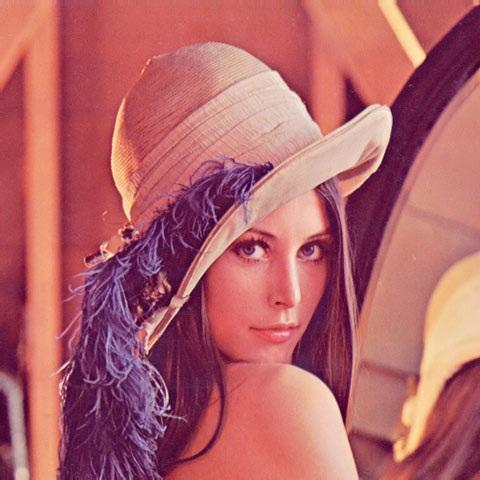
\includegraphics[width=40mm]{canny_original.jpg}
        \caption{Original}
    \end{minipage}%
    \begin{minipage}{.5\textwidth}
        \centering
        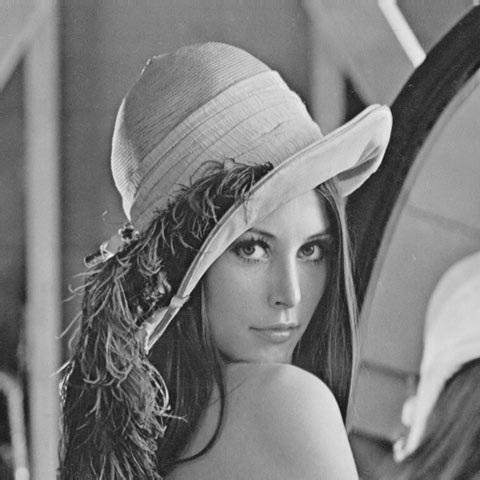
\includegraphics[width=40mm]{canny_grayscale.jpg}
        \caption{Grayscaled}
    \end{minipage}
\end{figure}


\subsubsection{Step 2: Apply Gaussian filter to smooth the image in order to remove the noise}
Since all edge detection results are easily affected by image noise, it is essential to filter out the noise to prevent false detection caused by noise. To smooth the image, a Gaussian filter is applied to convolve with the image.

\begin{figure}[!htb]
    \centering
    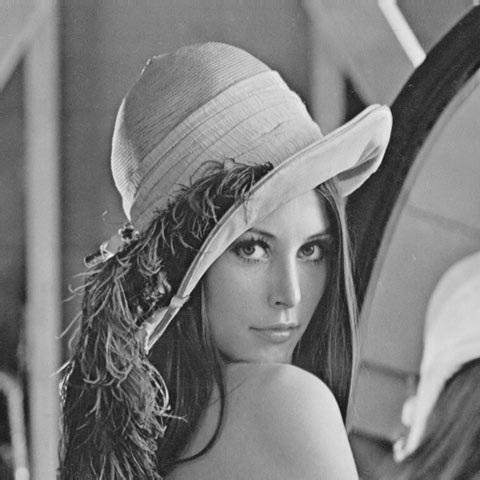
\includegraphics[width=40mm]{canny_grayscale.jpg}
    \caption{Gaussian blurred}
\end{figure}


\subsubsection{Step 3: Find the intensity gradients of the image}
An edge in an image may point in a variety of directions, so the Canny algorithm uses four filters to detect horizontal, vertical and diagonal edges in the blurred image. The edge detection operator (such as Roberts, Prewitt, or Sobel) returns a value for the first derivative in the horizontal direction ($G_{x}$) and the vertical direction ($G_{y}$). From this the edge gradient and direction can be determined. Here is an example of the sobel operator:

\begin{figure}[!htb]
    \centering
    \begin{minipage}{.5\textwidth}
        \centering
        $G_{x} = S_{x} * A =
        \left[ \begin{array}{rrr}
        1 & 0 & -1 \\
        2 & 0 & -2 \\
        1 & 0 & -1 \\
        \end{array}\right] $
    \end{minipage}%
    \begin{minipage}{.5\textwidth}
        \centering
        $G_{y} = S_{y} * A =
        \left[ \begin{array}{rrr}
        1 & 2 & 1 \\
        0 & 0 & 0 \\
        -1 & -2 & -1 \\
        \end{array}\right] $
    \end{minipage}
\end{figure}

\vspace{5mm}
\noindent Using the two operators you can then calculate the magnitude and the directional gradients of the image as follows:

\begin{figure}[!htb]
    \centering
    \begin{minipage}{.5\textwidth}
        \centering
        $|G| = \sqrt(G^{2}_{x} + G^{2}_{y})$
        \caption{Magnitude}
    \end{minipage}%
    \begin{minipage}{.5\textwidth}
        \centering
        $\Theta = arctan(G_{x}/G_{y})$
        \caption{Directinal gradients}
    \end{minipage}
\end{figure}

\vspace{5mm}
\noindent The resulting magnitude looks like:
\begin{figure}[!htb]
    \centering
    \begin{minipage}{.33\textwidth}
        \centering
        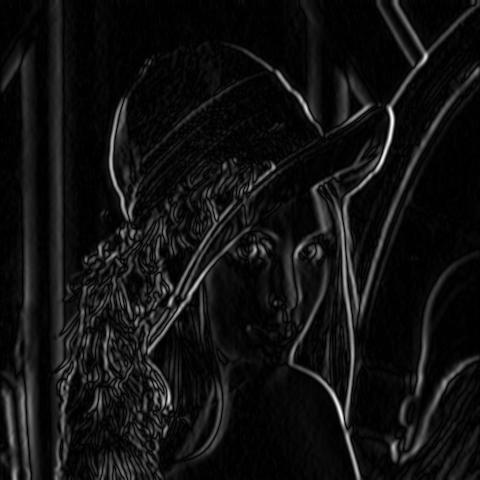
\includegraphics[width=40mm]{canny_sobel_x.jpg}
        \caption{$Sobel_{x}$}
    \end{minipage}%
    \begin{minipage}{.33\textwidth}
        \centering
        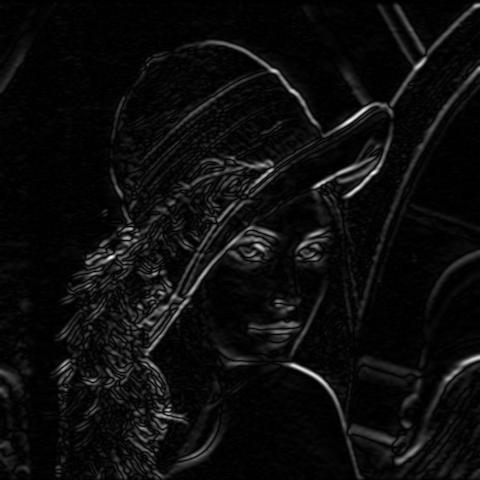
\includegraphics[width=40mm]{canny_sobel_y.jpg}
        \caption{$Sobel_{y}$}
    \end{minipage}
    \begin{minipage}{.33\textwidth}
        \centering
        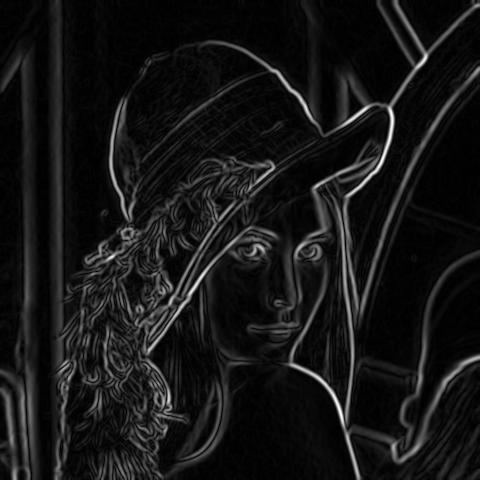
\includegraphics[width=40mm]{canny_magnitude.jpg}
        \caption{$Magnitude$}
    \end{minipage}
\end{figure}


\subsubsection{Step 4: Apply non-maximum suppression to get rid of spurious response to edge detection}
Non-maximum suppression is an edge thinning technique. After applying gradient calculation, the edge extracted from the gradient value is still quite blurred. Ideally, the final image should have only thin edges. Thus non-maximum suppression can help to suppress all the gradient values (by setting them to 0) except the local maxima, which indicate locations with the sharpest change of intensity value. The algorithm for each pixel in the gradient image is:

\begin{figure}[!htb]
    \centering
    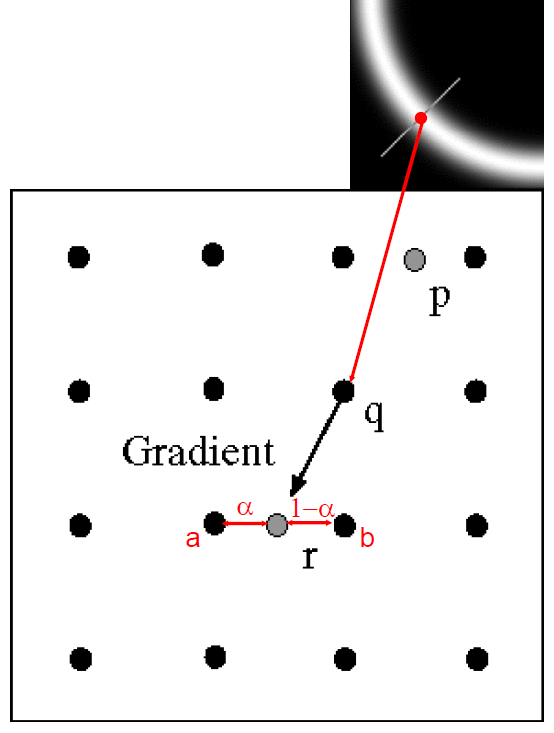
\includegraphics[width=40mm]{canny_nms_example.png}
\end{figure}


\noindent Non maximum suppression works by finding the pixel with the maximum value in an edge. In the above image, it occurs when pixel q has an intensity that is larger than both p and r where pixels p and r are the pixels in the gradient direction of q. If this condition is true, then we keep the pixel, otherwise we set the pixel to zero (make it a black pixel). Non maximum suppression can be achieved by interpolating the pixels for greater accuracy:

\begin{figure}[!htb]
    \centering
    $r = \alpha * b + (1 − \alpha) * a$
\end{figure}

\vspace{5mm}
\noindent Here is a resulting image:
\begin{figure}[!htb]
    \centering
    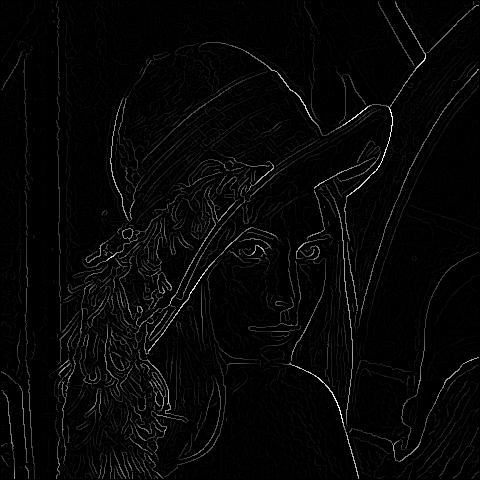
\includegraphics[width=45mm]{canny_nms.jpg}
    \caption{Non maximum suppression}
\end{figure}


\subsubsection{Step 5: Apply double threshold to determine potential edges}
After application of non-maximum suppression, remaining edge pixels provide a more accurate representation of real edges in an image. However, some edge pixels remain that are caused by noise and color variation. In order to account for these spurious responses, it is essential to filter out edge pixels with a weak gradient value and preserve edge pixels with a high gradient value. This is accomplished by selecting high and low threshold values. If an edge pixel’s gradient value is higher than the high threshold value, it is marked as a strong edge pixel. If an edge pixel’s gradient value is smaller than the high threshold value and larger than the low threshold value, it is marked as a weak edge pixel. If an edge pixel's value is smaller than the low threshold value, it will be suppressed. The two threshold values are empirically determined and their definition will depend on the content of a given input image.

\begin{figure}[!htb]
    \centering
    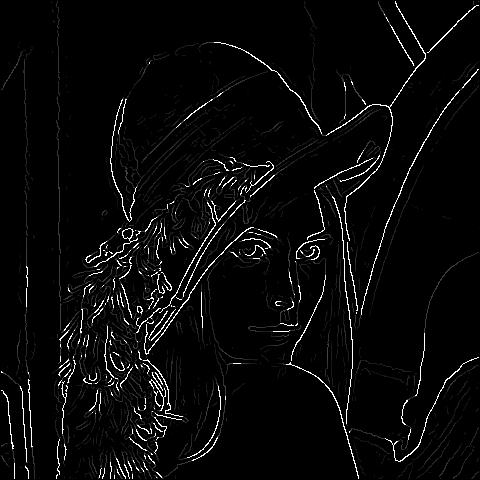
\includegraphics[width=40mm]{canny_double_thresholding.jpg}
    \caption{Double thresholding}
\end{figure}


\subsubsection{Step 6: Track edge by hysteresis: Finalize the detection of edges by suppressing all the other edges that are weak and not connected to strong edges}
So far, the strong edge pixels should certainly be involved in the final edge image, as they are extracted from the true edges in the image. However, there will be some debate on the weak edge pixels, as these pixels can either be extracted from the true edge, or the noise/colour variations. To achieve an accurate result, the weak edges caused by the latter reasons should be removed. Usually a weak edge pixel caused from true edges will be connected to a strong edge pixel while noise responses are unconnected. To track the edge connection, blob analysis is applied by looking at a weak edge pixel and its 8-connected neighbourhood pixels. As long as there is one strong edge pixel that is involved in the blob, that weak edge point can be identified as one that should be preserved.

\begin{figure}[!htb]
    \centering
    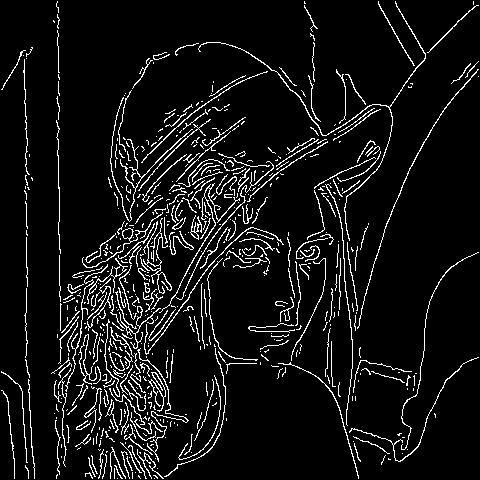
\includegraphics[width=40mm]{canny_final.jpg}
    \caption{Final Result from Canny Edge Detection Algorithm}
\end{figure}


%%%%%%%%%%%%%%%%%%%%%%%%%%%%%%%%%%%%%%%%%%%%%%%%%%%%%%%%%%%%%%%%%%%%%%%%%%%%%%%%%%%%%%%%%%%%%%%%%%%%


\subsection{What are the drawbacks of the original canny edge detector?}
While traditional Canny edge detection provides relatively simple but precise methodology for edge detection problem, with more demanding requirements on the accuracy and robustness on the detection, the traditional algorithm can no longer handle the challenging edge detection task. The main defects of the traditional algorithm can be summarized as follows:

\begin{itemize}
    \item Use an adaptive filter to apply different smoothing for noise and edge
    \item Select an optimal operator
    \item Use dynamic threshold values
    \item Use a better method for morphological detection
\end{itemize}

\cite{zhou11}

% \begin{enumerate}
%     \item A Gaussian filter is applied to smooth out the noise, but it will also smooth the edge, which is considered as the high frequency feature. This will increase the possibility of missing weak edges, and the appearance of isolated edges in the result.
%
%     As both edge and noise will be identified as high frequency signal, simple Gaussian filter will add smooth effect on both of them. However, in order to reach high accuracy of detection of the real edge, it is expected that more smooth effect should be added to noise and less smooth effect should be added to the edge. \cite{wang09} from Changsha University of Science and Technology developed an adaptive filter, where the filter will evaluate discontinuity between greyscale values of each pixel. The higher the discontinuity, the lower the weight value is set for the smooth filter at that point. Contrarily, the lower the discontinuity between the greyscale values, the higher the weight value is set to the filter.
%
%     \item For the gradient amplitude calculation, the old Canny edge detection algorithm uses the Centre in a small 2×2 neighbourhood window to calculate the finite difference mean value to represent the gradient amplitude. This method is sensitive to noise and can easily detect false edges and lose real edges.
%
%     The gradient magnitude and direction can be calculated with a variety of different edge detection operators, and the choice of operator can influence the quality of results. A very commonly chosen one is the 3x3 Sobel filter. However, other filters may be better by, such as a 5x5 Sobel filter which will reduce noise or the Scharr filter which has better rotational symmetry. Other common choices are Prewitt (used by \cite{zhou11}) and Roberts Cross.
%
%     \item In the traditional Canny edge detection algorithm, there will be two fixed global threshold values to filter out the false edges. However, as the image gets complex, different local areas will need very different threshold values to accurately find the real edges. In addition, the global threshold values are determined manually through experiments in the traditional method, which leads to complexity of calculation when a large number of different images need to be dealt with.
%
%     In order to resolve the challenges where it is hard to determine the dual-threshold value empirically, Otsu's method (\cite{otsu78}) can be used on the non-maximum suppressed gradient magnitude image to generate the high threshold. The low threshold is typically set to 1/2 of the high threshold in this case. Since the gradient magnitude image is continuous-valued without a well-defined maximum, Otsu's method has to be adapted to use value/count pairs instead of a complete histogram.
%
%     \item The result of the traditional detection cannot reach a satisfactory high accuracy of single response for each edge - multi-point responses will appear.
%
%     While the traditional canny edge detection have implemented a good detection result to meet with the first two criteria, it does not meet with the single response per edge strictly. A mathematical morphology to thin the detected edge is developed by \cite{zhong92}.
% \end{enumerate}


%%%%%%%%%%%%%%%%%%%%%%%%%%%%%%%%%%%%%%%%%%%%%%%%%%%%%%%%%%%%%%%%%%%%%%%%%%%%%%%%%%%%%%%%%%%%%%%%%%%%


\subsection{What filter operators do you know?}
As a rule if you define your custom operator, the sum of all numbers should yield 0.
\subsubsection{Sobel operator}

\begin{figure}[!htb]
    \centering
    \begin{minipage}{.5\textwidth}
        \centering
        $G_{x} = S_{x} * A =
        \left[ \begin{array}{rrr}
        1 & 0 & -1 \\
        2 & 0 & -2 \\
        1 & 0 & -1 \\
        \end{array}\right] $
    \end{minipage}%
    \begin{minipage}{.5\textwidth}
        \centering
        $G_{y} = S_{y} * A =
        \left[ \begin{array}{rrr}
        1 & 2 & 1 \\
        0 & 0 & 0 \\
        -1 & -2 & -1 \\
        \end{array}\right] $
    \end{minipage}
\end{figure}


\subsubsection{Roberts cross}

\begin{figure}[!htb]
    \centering
    \begin{minipage}{.5\textwidth}
        \centering
        $\left[ \begin{array}{rr}
        1 & 0 \\
        0 & -1 \\
        \end{array}\right] $
    \end{minipage}%
    \begin{minipage}{.5\textwidth}
        \centering
        $\left[ \begin{array}{rr}
        0 & 1 \\
        -1 & 0 \\
        \end{array}\right] $
    \end{minipage}
\end{figure}

\subsubsection{Prewitt operator}

\begin{figure}[!htb]
    \centering
    \begin{minipage}{.5\textwidth}
        \centering
        $G_{x} = S_{x} * A =
        \left[ \begin{array}{rrr}
        1 & 0 & -1 \\
        1 & 0 & -1 \\
        1 & 0 & -1 \\
        \end{array}\right] $
    \end{minipage}%
    \begin{minipage}{.5\textwidth}
        \centering
        $G_{y} = S_{y} * A =
        \left[ \begin{array}{rrr}
        1 & 1 & 1 \\
        0 & 0 & 0 \\
        -1 & -1 & -1 \\
        \end{array}\right] $
    \end{minipage}
\end{figure}

\subsubsection{Laplace operator}

\begin{figure}[!htb]
    \centering
    \begin{minipage}{.5\textwidth}
        \centering
        $G_{xy} = S_{xy} * A =
        \left[ \begin{array}{rrr}
        0 & 1 & 0 \\
        1 & -4 & 1 \\
        0 & 1 & 0 \\
        \end{array}\right] $
    \end{minipage}%
    \begin{minipage}{.5\textwidth}
        \centering
        $G_{y} = S_{y} * A =
        \left[ \begin{array}{rrr}
        1 & 1 & 1 \\
        1 & -8 & 1 \\
        1 & 1 & 1 \\
        \end{array}\right] $
    \end{minipage}
    \caption{In addition to the first operator, this one detects 45°-edges}
\end{figure}


%%%%%%%%%%%%%%%%%%%%%%%%%%%%%%%%%%%%%%%%%%%%%%%%%%%%%%%%%%%%%%%%%%%%%%%%%%%%%%%%%%%%%%%%%%%%%%%%%%%%


\subsection{What is blob Connected-component labeling?}
Connected-component labeling is applied in the canny edge algorithm and it is an algorithmic application of graph theory, where subsets of connected components are uniquely labelled based on a given heuristic. In other words, it is used to detect connected regions in binary digital images.

\chapter{C++}

%% Topics:
%
% Inheritance
% Key-Words
% General Concepts
% Testing

\section{Theoretical Part}

\subsection{Inheritance}
\subsubsection{Write down an example inheritance class}
\begin{lstlisting}
    class C:  public D {
    };

    class B:  public D {
    };

    class A: public B, public C {
    };
\end{lstlisting}

\subsection{Key-Words}
\subsection{General Concepts}
\subsection{Testing}





\section{Practical Part}


%
%
% \subsection{What does the "static" keyword mean?}
% Static elements are independent of class instances and exist during during the entire application run-time. That said, they behave like global variables, but are visible (if set private) only in the scope of their class
%
%
%
% How do you declare virtual inheritance? Write down a code example.
% class C:  virtual public D {
% };
%
%
% \subsubsection{What is Doxygen?}
% Doxygen is the de facto standard tool for generating documentation (API) from annotated C++ sources, but it also supports other popular programming languages such as Java, Python and others.
%
% Link: http://www.doxygen.nl/manual/docblocks.html#specialblock
%
%
%
%
%
% \subsubsection{How do you write a gTest?}
% TEST(TestSuiteName, TestName) {
%   ... test body ...
% }
%
% For example, let's take a simple integer function:
%
% int Factorial(int n);  // Returns the factorial of n
% A test case for this function might look like:
%
% // Tests factorial of 0.
% TEST(FactorialTest, HandlesZeroInput) {
%   EXPECT_EQ(Factorial(0), 1);
% }
%
% // Tests factorial of positive numbers.
% TEST(FactorialTest, HandlesPositiveInput) {
%   EXPECT_EQ(Factorial(1), 1);
%   EXPECT_EQ(Factorial(2), 2);
%   EXPECT_EQ(Factorial(3), 6);
%   EXPECT_EQ(Factorial(8), 40320);
% }
%
%
%
%
% \subsubsection{What is a static variable definition?}
% A static variable is kept in the same memory location for the execution of the program. So the value is live for life of the execution.
%
%
% \subsubsection{What is a static member variable?}
% A static member variable means that the variable is shared between all instances of the class.
% That means, instead of each instance having a copy of the variable, all instances share this variable. It is often preferred to save space especially when the variable is an object of a class. Likewise for static functions and classes. There is only one copy of the variable. The idea is that creating and cleaning up the instances can be a computationally expensive process, if it can be made static, it is a good idea to speed up execution of the program.
% On the flip side, it can also be expensive to use a static variable. If using a static variable requires the CPU to fetch the variable from slower memory, rather than having it in the cache or stack. Each fetch from slower memory slows down execution time.
%
% \subsubsection{What is the difference between sign und unsigned numbers?}
% The "signed" indicator means that the item can hold positive or negative values. "Unsigned" doesn't distinguish between positive and negative values. A signed/unsigned variable can refer to any numerical data type (such as binary, integer, float, etc). Each data type might be further defined as signed or unsigned.
%
% For example, an 8-bit signed binary could hold values from 0-127, both positive and negative (1 bit is used for the sign and 7 bits for the value), while an 8-bit unsigned binary could hold values from 0-255 (nothing distinguishes whether or not the value should be considered positive or negative, though it is commonly assumed to be positive).
%
% A signed binary is a specific data type of a signed variable.
%
%
% https://www.toptal.com/c-plus-plus/interview-questions#iquestion_form
%
% https://www.tutorialspoint.com/cplusplus/cpp_questions_answers.htm

\chapter{   Deep Learning}
% CHAPTER SETTINGS
\graphicspath{{./images/computer_vision/}}

\section{Rgularization}

\subsection{Why do we use regularization?}
Regularization helps us control our model capacity, ensuring that our models are better at
making (correct) classifications on data points that they were not trained on, which we call the
ability to generalize. If we don’t apply regularization, our classifiers can easily become too complex
and overfit to our training data, in which case we lose the ability to generalize to our testing data
(and data points outside the testing set as well, such as new images in the wild).
However, too much regularization can be a bad thing. We can run the risk of underfitting, in
which case our model performs poorly on the training data and is not able to model the relationship
between the input data and output class labels (because we limited model capacity too much). For
example, consider the following plot of points, along with various functions that fit to these points.

addfigure starterbundle p.114




What we are doing here is looping over all entries in the matrix and taking the sum of squares.
The sum of squares in the L2 regularization penalty discourages large weights in our matrixW,
preferring smaller ones. Why might we want to discourage large weight values? In short, by
penalizing large weights, we can improve the ability to generalize, and thereby reduce overfitting.
Think of it this way – the larger a weight value is, the more influence it has on the output
prediction. Dimensions with larger weight values can almost singlehandedly control the output
prediction of the classifier (provided the weight value is large enough, of course) which will almost
certainly lead to overfitting.



\section{Activation Functions}


\section{Perceptron}
\chapter{Machine Learning}

\include{chapters/match}
\chapter{Natural Phenomena}

\chapter{   Tooling}
% CHAPTER SETTINGS
\graphicspath{{./images/tooling/}}

\section{Cmder}

\subsection{How do you change lambda promt?}
On windows, if you are using anaconda, there might be a problem with activating virtualenv, since conda does't not recognize the lambda character. Thus you have to change the lambda character in the cmder as follows:

\vspace{4mm}

\begin{lstlisting}
vim vendor/git-for-windows/etc/profile.d/git-prompt.sh
\end{lstlisting}


%%%%%%%%%%%%%%%%%%%%%%%%%%%%%%%%%%%%%%%%%%%%%%%%%%%%%%%%%%%%%%%%%%%%%%%%%%%%%%%%%%%%%%%%%%%%%%%%%%%%


\section{Anaconda}

\subsection{How do you handle virtual environment in anaconda}
\begin{lstlisting}
    # create virtual environment
    conda create -n myenv python=3.4

    # activate the virtual environment
    # windows
    source activate myenv

    # deactivate the virtual environment
    conda deactivate

    # print all virtual environments
    # * indicates the active one
    conda info --envs

    # delete virtual environment
    conda remove --name myenv --all
\end{lstlisting}


%%%%%%%%%%%%%%%%%%%%%%%%%%%%%%%%%%%%%%%%%%%%%%%%%%%%%%%%%%%%%%%%%%%%%%%%%%%%%%%%%%%%%%%%%%%%%%%%%%%%


\section{PyCharm}

\subsection{Pylint setup}

pylint is used for static code analysis.

To create a shortcut for the code analysis in pycharm:

\begin{enumerate}
    \item File → Settings
    \item Tools → External Tools
    \item Click the "+" Sign to add a new Tool
    \item Enter the following:
    \begin{itemize}
        \item Name: pylint
        \item Description: pylint code inspection
        \item Program: \$PyInterpreterDirectory\$\textbackslash pylint.exe
        \item Arguments: -v --rcfile=.pylintrc "--msg-template='{abspath}:{line:5d},{column:2d}: {msg} ({symbol})'" --output-format=colorized "\$FilePath\$"
        \item Working directory: \$ProjectFileDir\$
        \item Advanced Options
        \begin{itemize}
            \item Synchronize files after execution: True
            \item Open Console for tool Output: True
            \item Output filters: \$FILE_PATH\$:\textbackslash %s*\$LINE\$\textbackslash,\textbackslash s*\$COLUMN\$:
        \end{itemize}
    \end{itemize}
\end{enumerate}

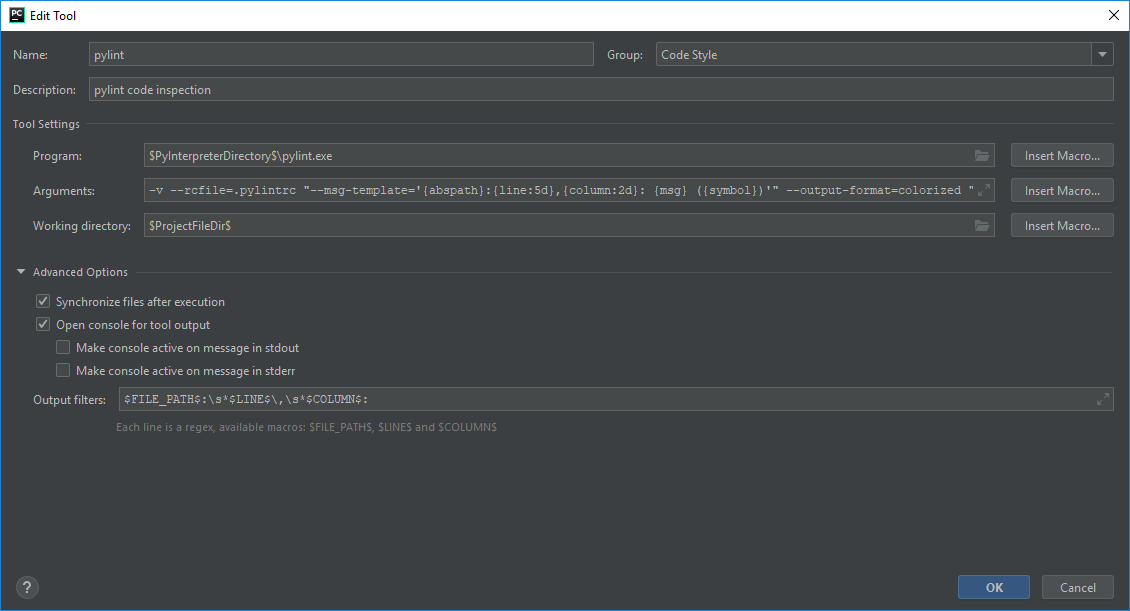
\includegraphics[width=120mm]{pycharm_pylint_setup.png}


%%%%%%%%%%%%%%%%%%%%%%%%%%%%%%%%%%%%%%%%%%%%%%%%%%%%%%%%%%%%%%%%%%%%%%%%%%%%%%%%%%%%%%%%%%%%%%%%%%%%


\subsection{bandit setup for security testing}

Testing security: bandit
bandit is used to check for common security vulnerabilities

To create a shortcut for the code analysis in pycharm:

% \begin{enumerate}
%     \item File → Settings
%     \item Tools → External Tools
%     \item Click the "+" Sign to add a new Tool
%     \item Enter the following:
%     \begin{itemize}
%         \item Name: bandit
%         \item Description: Linter for security vulnerabilities
%         \item Program: $PyInterpreterDirectory$\bandit
%         \item Arguments: -r "$FilePath$"
%         \item Working directory: $ProjectFileDir$
%         \item Advanced Options
%         \begin{itemize}
%             \item Syncronize files after execution: True
%             \item Open Console for tool Output: True
%             \item Output filters: \s*Location:\s*$FILE_PATH$:\s*$LINE$
%         \end{itemize}
%     \end{itemize}
% \end{enumerate}



\subsection{yapf setup}
Automatic Code Formatting: yapf
yapf is used for automatic code formatting.

To create a shortcut for the code analysis in pycharm:

% \begin{enumerate}
%     \item File → Settings
%     \item Tools → External Tools
%     \item Click the "+" Sign to add a new Tool
%     \item Enter the following:
%     \begin{itemize}
%         \item Name: yapf in-place
%         \item Description: Reformat Code in-place
%         \item Program: $PyInterpreterDirectory$\yapf.exe
%         \item Arguments: --style=yapf.conf -i "$FilePath$"
%         \item Working directory: $ProjectFileDir$
%         \item Advanced Options
%         \begin{itemize}
%             \item Syncronize files after execution: True
%             \item Open Console for tool Output: True
%         \end{itemize}
%     \end{itemize}
% \end{enumerate}



If you don't want to replace the code in-place remove the -i argument and add another config for that (Lächeln)


%%%%%%%%%%%%%%%%%%%%%%%%%%%%%%%%%%%%%%%%%%%%%%%%%%%%%%%%%%%%%%%%%%%%%%%%%%%%%%%%%%%%%%%%%%%%%%%%%%%%

\section{PostgreSQL}

% get it here from the file

%%%%%%%%%%%%%%%%%%%%%%%%%%%%%%%%%%%%%%%%%%%%%%%%%%%%%%%%%%%%%%%%%%%%%%%%%%%%%%%%%%%%%%%%%%%%%%%%%%%%


%\appendix
%\printindex

\bibliography{bib/papers}

\end{document}

% todo:
% remove Theoretical and Practical parts
% allowed only subsections
% use the input command to make the document more uebersichtlicher
% move the sections to a separate file
% get the script up and running
